% "Brief" explanation of the Schwarz-Christoffel transform
% David Lawrence Miller
% d.l.miller@bath.ac.uk
 
% Started : 29 October 2008
 
\documentclass[a4paper,10pt]{amsart}
 
% Load some packages
\usepackage{times, amsmath, amssymb, amsfonts, url, natbib, bm, rotating}
 
\usepackage{multirow}
\usepackage{graphicx}

% top matter
\title{Technical details of the schwarz-christoffel transform in relation to its application to smoothing}
\author{David Lawrence Miller}
\email{d.l.miller@bath.ac.uk}
\address{Mathematical Sciences, University of Bath, Bath, United Kingdom}
 
% Shortcuts
% Probability
\newcommand{\prob}[1]{\mathbb{P}\left[ #1 \right]}
% Hovitz-Thompson
\newcommand{\HT}{\hat{\tau}_{HT}}
% Schwarz-Christoffel
\newcommand{\sch}{Schwarz-Christoffel }
% fprime
\newcommand{\fprime}{f^\prime(z)}
% figure reference command
\newcommand{\fig}[1]{\emph{fig.} (\ref{#1})}
% equation reference command
\newcommand{\eqn}[1]{\emph{eqn.} (\ref{#1})}
% phi inverse
\newcommand{\phiinv}{\phi^{-1}}
% use other phi
\renewcommand{\phi}{\varphi}

\begin{document}
 
% The abstract
\begin{abstract}
This document lays out some of the technical details of the \sch mapping from a statistical perspective for the purposes of using the transform to morph a 2D region before performing smoothing over it. 
\end{abstract}
 
 
% New theorem for theorems
\newtheorem{thm}{Theorem}[section]
 
%New theorem for definitions
\newtheorem{defn}{Definition}[section]
 
\maketitle

\markright{TECH. DETAILS OF SCHWARZ-CHRISTOFFEL MAPPING}

\section{Method}

Given some complicated region that it is difficult to smooth over, one approach is to morph or transform the domain. So, for example, one could transform a region into a rectangle, circle or other familiar shape to avoid the problems such as leakage. In this spirit, we wish to find some mapping such as $\phi$ in \fig{simpledia}.

% Simple diagram showing the mapping
\begin{figure} [htbp]
\centering
\includegraphics[scale=0.3]{figs/simpledia.pdf}
\caption{The function $\phi$ takes the points in the rectangle and maps them to the region on the left.}
\label{simpledia}
\end{figure}

In our case we use a method from complex analysis called the \sch mapping. This takes some arbitrary polygon and maps it to some set shape. Commonly this is the upper half-plane ($H^+$), a rectangle or the unit disk. 

This is achieved in the $H^+$ case by taking the vertices of the polygon and mapping them to points on the real line (see \fig{reallinedia}.) This can be thought of as ``unwrapping'' the polygon onto the real line. 

For the unit disk case, we take points on the circle bounding the unit disk and map vertices on the polygon to those points (see \fig{unitdiskdia}.) One can think of this as adding control points to the unit circle and using the exponents in the \sch formula (below) to tighten up the angles.

The rectangular case is somewhat similar to the unit disk in that extra points are added to the boundary and the angles of these points tightened until the shape is identical to the polygon.

% Diagram showing upper half plane to polygon
\begin{figure} [tbp]
\centering
\includegraphics[scale=0.6]{figs/reallinedia.pdf}
\caption{Here we show the mapping of the upper half-plane to the polygon. The vertices ($w_k$) are the result of applying $\phi$ to the points on the real line ($w^*_k$). The boundry of the polygon is mapped to the real line. Note that the final vertex, $w^*_6$ is mapped to the point $\infty$ on the real line.}
\label{reallinedia}
\end{figure}

% Diagram showing unit disk to polygon
\begin{figure} [tbp]
\centering
\includegraphics[scale=0.6]{figs/unitdiskdia.pdf}
\caption{We now have the same situation as in \fig{reallinedia}, except that now the boundry of the polygon is mapped to the boundry of the unit disk.}
\label{unitdiskdia}
\end{figure}


\subsection{Nomenclature}

We first define a polygon formally and its associated quantities as they will be referred to throughout the rest of the document.

A polygon, $\Gamma$, is a collection of vertices $w_1, w_2,\dots,w_n$ and interior angles $\alpha_1\pi, \alpha_2\pi, \dots, \alpha_n\pi$. For convenience we define $w_{n+1} = w_1$ and $w_0=w_n$. Numbering of vertices is anti-clockwise. The angles are such that $\alpha_k \in (0,2]$ and we require:

\begin{equation}
\sum_{k=1}^n (1-\alpha_k) = 2.
\end{equation}

We also define the exterior angle, $\theta_k\pi$, as given by $(1-\alpha_k)\pi$ (see \fig{anglediagram}.) It is the exterior angle that is of interest to us here.

% Diagram showing the exterior/interior angle relationship.
\begin{figure} [bp]
\centering
\includegraphics[scale=0.6]{figs/anglediagram.pdf}
\caption{The external angle $\theta_k$ is associated with the vertex $w_k$. The internal angle is given by $\alpha_k$.}
\label{anglediagram}
\end{figure}

Here we use $\Gamma$ to refer to the boundary of the polygon and $P$ to the region inside. We refer to two domains the $W$ and the $W^*$, denoting the original domain (of $\Gamma$) and the transformed domain (of the plane, unit disk or rectangle) respectively. 

Vertices on the polygon are denoted as $w_k$ and those in the transformed domain are denoted as $w^*_k$ (referred to as \emph{prevertices}.) In general a point in the polygon's original domain is denoted as $w$ and in the transformed domain as $w^*$.

We use the function $\phi$ to go from the transformed domain to the polygon (from $W^*$ to $W$). The inverse of $\phi$, $\phi^{-1}$, is used to go from the polygon to the disk, rectangle or half-plane (from $W$ to $W^*$.)  See \fig{mappingdia}.

% Mapping diagram from my whiteboard
\begin{figure} [tbp]
\centering
\includegraphics[scale=0.5]{figs/mappingdia.pdf}
\caption{Diagram showing the forwards and backwards mappings.}
\label{mappingdia}
\end{figure}


\section{\sch Mapping}

We now look at the mathematical formulation for the upper half-plane, unit disk and rectangle. There are many mappings that can be performed however those detailed here are either cannonical (in the case of the half-plane) or considered to be useful in a smoothing context (the other two.) For the purposes of smoothing we are interested in the function $\phi^{-1}$ (\emph{ie.} the function that goes from our domain to the transformed one.) We must first calculate $\phi$ before we may calculate its inverse\footnote{In conformal mapping literature $\phi$ is referred to as the \emph{forwards map} and $\phi^{-1}$ as the \emph{backwards map}.}.

The forwards map, $\phi$, as we will see below, is determined up to translation, scaling, and rotation by the prevertices. So, our task is to efficiently find the prevertices and hence find the mapping $\phi$. The task of obtaining the prevertices is known as the \emph{\sch parameter problem}.


\subsection{The upper half-plane}

When we map $\Gamma$ to $H^+$ we set $\phi(\infty) = w_n$ without any loss of generality. We then have the formula:

\begin{equation}
\phi(w^*) = A + C \int^{w^*}_{w^*_0} \prod_{k=1}^{n-1} (\zeta-w^*_k)^{-\theta_k} d\zeta.
\end{equation}

Here $A$ and $C$ are complex constants determined once the $w^*_k$ have been calculated. These control the scaling and rotation of the transform.

Although setting $\phi(\infty) = w_n$ does not make any difference in a mathematical sense, it does mean that the density of the points mapped into $H^+$ is rather odd. Given two adjacent points near $w_n$, their spacing on the upper half-plane is huge in comparison to two adjacent points near the other vertices. For this reason it is more common to use the unit disk or rectangle mapping. 

\subsection{Unit disk}

The formula for the unit disk looks very similar to that for $H^+$ but the product now runs over all prevertices. The integrand is simply a constant multiple of the $H^+$ case. This is merely to avoid problems in the calculation of the branch cuts (\cite{driscoll}, \emph{p. 12}).

\begin{equation}
\label{unitscmap}
\phi(w^*) = A + C \int^{w^*}_{w^*_0} \prod_{k=1}^{n} (1 - \frac{\zeta}{w^*_k})^{-\theta_k} d\zeta.
\end{equation}

As above, $A$ and $C$ are complex constants.

\subsection{Rectangle}
For the rectangle case we must specify four vertices of $\Gamma$ that map to the four corners of the rectangle. This uniquely specifies the aspect ratio of the rectangle (\cite{driscoll}, \emph{p. 48}).

The rectangle mapping is slightly different in its calculation to the two above mappings. We first map $\Gamma$ to the upper half-plane as detailed above. From there we can use the Jacobi elliptic function\footnote{The form of which is $\int_0^\gamma \frac{dt}{\sqrt{1-k^2\sin^2t}}$. Further details may be found at \url{http://mathworld.wolfram.com/JacobiEllipticFunctions.html}.} to map a rectangle to the upper half-plane. The computation of this map is expensive due to the evaluation of the elliptic function (\cite{driscoll}, \emph{p. 49}) so a shortcut using the mapping to the mapping to the strip. We do not go into further about detail here (as the computational intricacies are covered in \cite{howell90}.)



\section{Computation of the \sch mapping}

To compute the map, we need to find the prevertices\footnote{Since the complex constants just control scaling and rotation, we can compute them after computing the $w^*_k$.}, $w^*_k$. We achieve this iteratively by approximating the $w^*_k$ then mapping those points back to the polygon to give an estimate of $\Gamma$, $\Gamma^\prime$. 

To measure the quality of approximation of $\Gamma^\prime$ to $\Gamma$ we use the following set of equations:

\begin{equation}
\label{optimizeme}
\frac{\vert \phiinv(w^*_{k+1}) -  \phiinv(w^*_k) \vert}{\vert \phiinv(w^*_2)-\phiinv(w^*_1)\vert} - \frac{\vert w_{k+1} - w_k\vert}{\vert w_2 - w_1\vert} = 0, \qquad \text{for } k=3,\dots,n-1.
\end{equation}

Here $\vert \phiinv(w^*_{k+1}) -  \phiinv(w^*_k) \vert$ is the distance between the $k^{th}$ and $(k+1)^{th}$ vertex.  We find this by integrating along the line between the points within $W$.

Intuitively, we are comparing the side lengths of the polygon in order to evaluate approximation of $\Gamma$ in each iteration (\cite{snider}, \emph{p. A-3}), both scaled by the distance between the first two vertices (in their respective domains.)

Note that the relation does not include the vertex $w_n$, nor do we look at $w_1$ or $w_2$ in the numerator on the right of the above equation. The former is since (by theorem 3.1 of \cite{driscoll}, \emph{p. 24}) a polygon is precisely defined by its angles and its vertices not including $w_n$\footnote{Since we know the direction of the edges leaving $w_1$ and $w_{n-1}$, we may find the point where they meet.}. The latter is due to all vertices (and hence $w_1$ and $w_2$) being rescaled and translated by the complex constants, $A$ and $C$, in the \sch formula.

It is for this reason, in the upper half-plane case, that we can map $w_n$ to $\infty$ without loss of generality. In practice we fix $w^*_n=1$, $w^*_{n-1}=-i$ and $w^*_{n-2}=-1$ in the unit disk case (\cite{driscoll}, \emph{p. 24}.) For the rectangle case we need to specify which vertices of $\Gamma$ map to which vertices of the rectangle.

We may find the scaling factor, $C$, (from \eqn{unitscmap}) by using the following equation:

\begin{equation}
C=\frac{\vert \phiinv(w^*_2)-\phiinv(w^*_1)\vert}{\vert w_2 - w_1\vert},
\end{equation}

otherwise, we can assume that up to scaling and rotation that $w_1$ and $w_2$ are correct. In which case we know that $\Gamma$ and $\Gamma^\prime$ are similar (in the geometric sense.) 

$A$ is the image of the base point of the integration and is usually written as $w_0$. For computational reasons this is usually the prevertex nearest to the point $w^*$ that we wish to map in \eqn{unitscmap}  (\cite{driscoll}, \emph{p. 27}.)


\subsection{Sketch of an algorithm to calculate the \sch mapping}
\label{algorithmsketch}
\begin{enumerate}
\item Accept inputs:
   \begin{enumerate} 
      \item $w_1,\dots,w_n$ (the vertices),
      \item $n$ (the number of vertices),
      \item $\theta_1,\dots,\theta_n$ (the external angles at each vertex).
   \end{enumerate}
\item Define the objective function, $F$, as:
 \begin{equation*}
F=\frac{\vert \phi^{-1}(w^*_{k+1}) -  \phi^{-1}(w^*_k) \vert}{\vert \phi^{-1}(w^*_2)-\phi^{-1}(w^*_1)\vert} - \frac{\vert w_{k+1} - w_k\vert}{\vert w_2 - w_1\vert}, \qquad \text{for } k=3,\dots,n-1,
 \end{equation*}
\item Use steepest descent and then Newton's method to until $\vert F\vert < \epsilon \quad \forall k$. \item Calculate $C$ and $A$ as detailed above.
\item Return values for $w^*_1,\dots,w^*_n$, $C$ and $A$.
\end{enumerate}


Starting values for the algorithm are evenly spaced vertices around the edge of the disk/rectangle or, in the case of the plane, along the real line. This is, of course, apart from those points specified as fixed (see above.)

\subsection{Getting between $W$ and $W^*$}

\subsubsection{Forwards map}

Calculating the forwards map is simply a case of evaluating $\phi$ at the necessary points. If we wish to find the point on polygon ($w$), given we know the point on the disk ($w^*$), we compute:

\begin{equation}
\label{forwardsmap}
w=\phi(w^*) = w_0 + C \int_{w^*_0}^{w^*} \prod_{k=1}^{n} (1 - \frac{\zeta}{w^*_k})^{-\theta_k} d\zeta,
\end{equation}

where $w^*_0$ is any point in the closed disk such that $w_0 = \phi(w^*_0)$ is known and non-infinite. We may choose any point since the integrand is analytic throughout the mapping and hence the integral is path-independent (\cite{driscoll} \emph{p. 27}). A common choice for $w_0$ is the centre of the polygon.

Equivalent expressions exist for the rectangle and upper half-plane cases.


\subsubsection{Backwards map}

To calculate points from the polygon to points on the unit disk, there are two possible approaches: \emph{1)} using Newton's method to solve the equation $\phi(w^*)-w=0$ and \emph{2)} solving the IVP:

\begin{equation}
\label{scivp}
\frac{dw^*}{dw}=\frac{1}{\phi^{-1}(w^*)} \quad \text{and} \quad \phiinv(w_0)=w^*_0.
\end{equation}

We in fact use a combination of these methods; solving (\ref{scivp}) approximately gives the starting values for the Newton iterations which are significantly faster (since $\phi^{-1}$ is cheaper to compute than $\phi$.) (\cite{driscoll} \emph{p. 29}.)

The only problem with this is that the path from $w_0$ to the point to map, $w$, must lie entirely inside the polygon. This is not known since after the mapping has been computed, the only points that are known are the vertices (at which the IVP is singular.) So, to combat this, all of the points on the path are checked sequentially. This computation, although inelegant, is fast compared to the IVP/Newton iterations.

An example of using the backwards map to find the transformed co-ordinates from a square to the unit disk is given in \fig{squaredomain}. An irregular nonagon is given in \fig{irregdomain}.


% Square domain mapping diagram
\begin{figure} [bp]
\centering
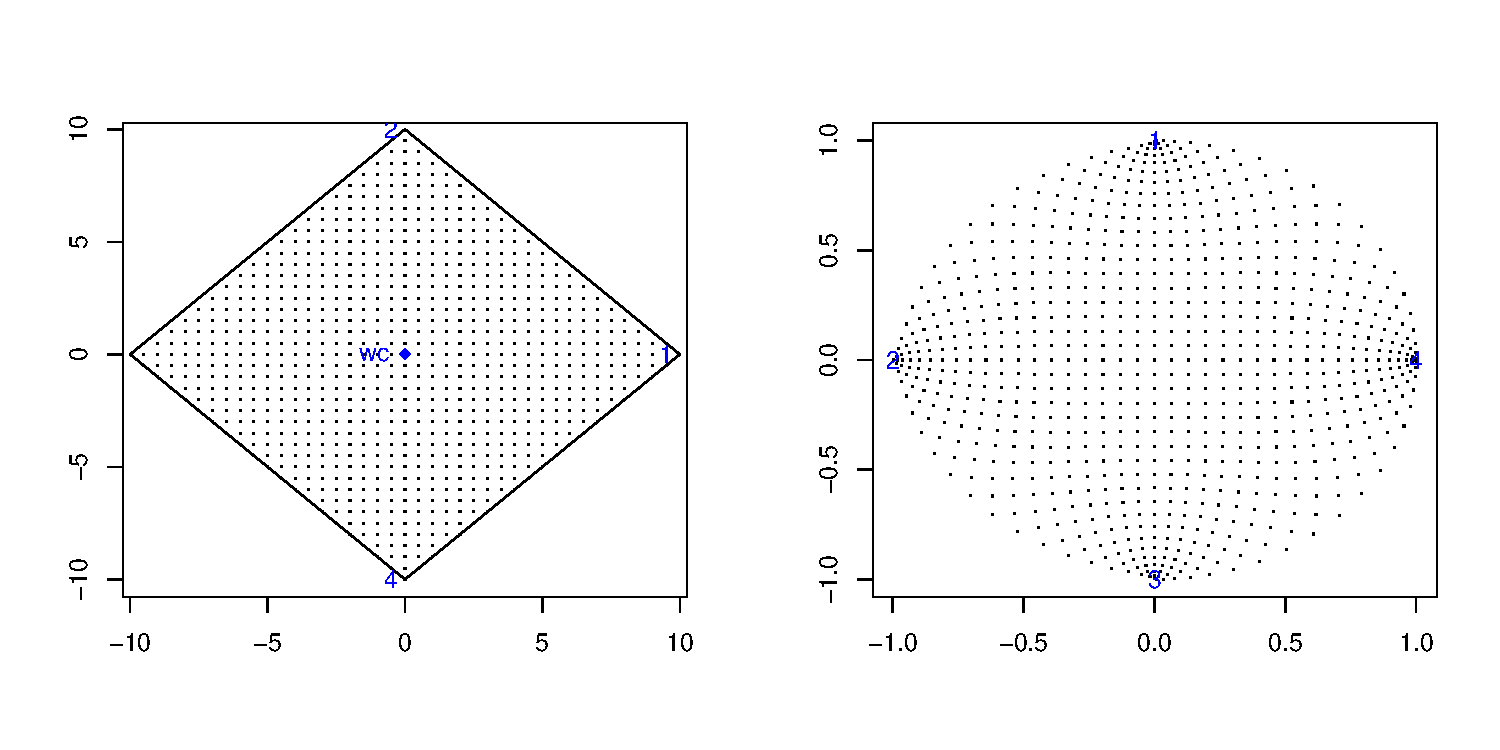
\includegraphics[scale=0.5]{figs/squaredomain.pdf}
\caption{The left panel shows a regular grid of points over the square region. The right panel shows the mapping of these points under the \sch transformation to the unit disk.}
\label{squaredomain}
\end{figure}

% Irregular mapping diagram
\begin{figure} [tbp]
\centering
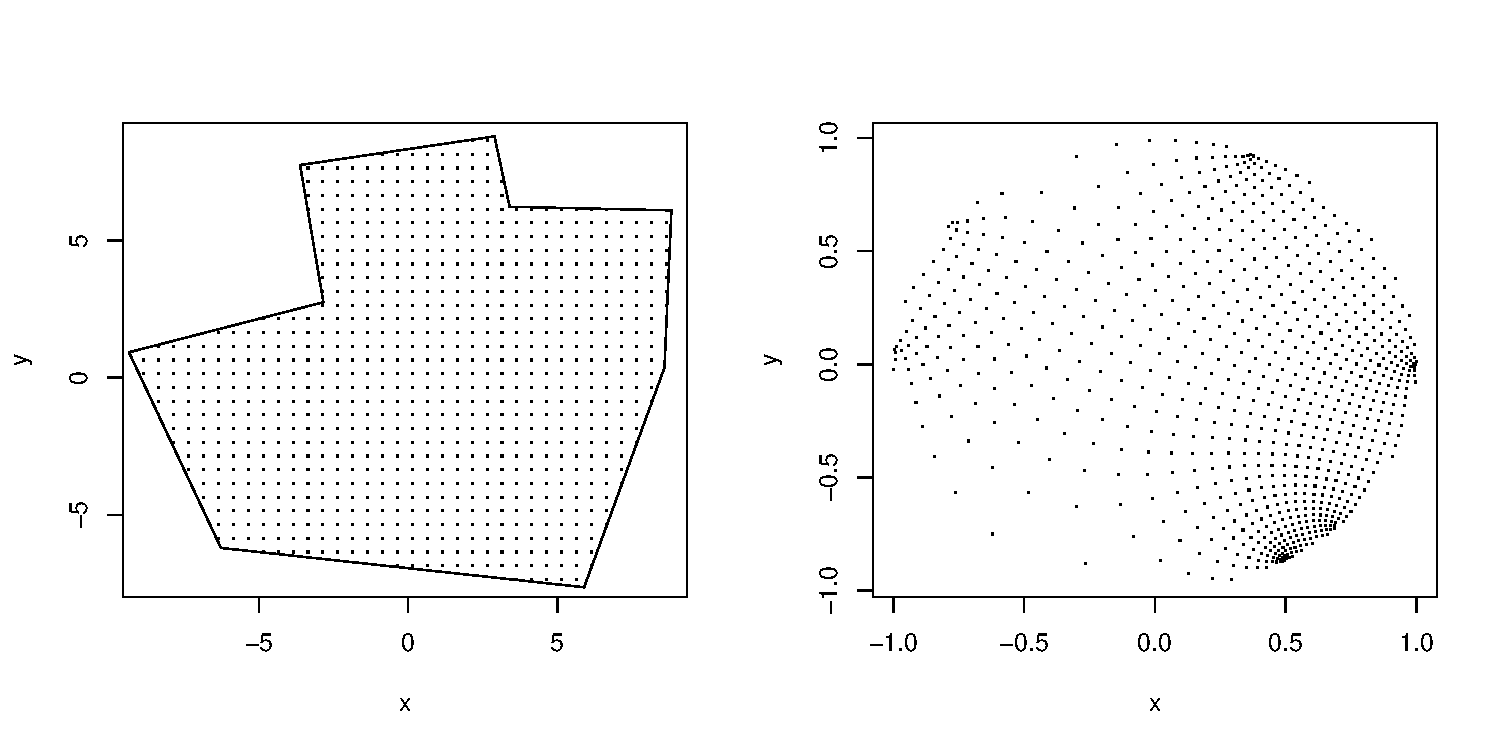
\includegraphics[scale=0.5]{figs/irregulardomain.pdf}
\caption{The left panel shows a regular grid of points over region bound by a irregular nonagon. The right panel shows the mapping of these points under the \sch tranformation to the unit disk.}
\label{irregdomain}
\end{figure}

\section{Crowding}

\subsection{The crowding problem}
When the polygon is elongated or has many vertices, the mapped vertices are positioned too closely in the transformed domain. This effect is referred to as \emph{crowding} and can be observed in \fig{crowdeddisk}. Indeed, \cite{howell90} points out that in elgonated regions prevertices can be located exponentially close such that in finite precision arithmetic they have merged.

% Crowded mapping diagram
\begin{figure} [tbp]
\centering
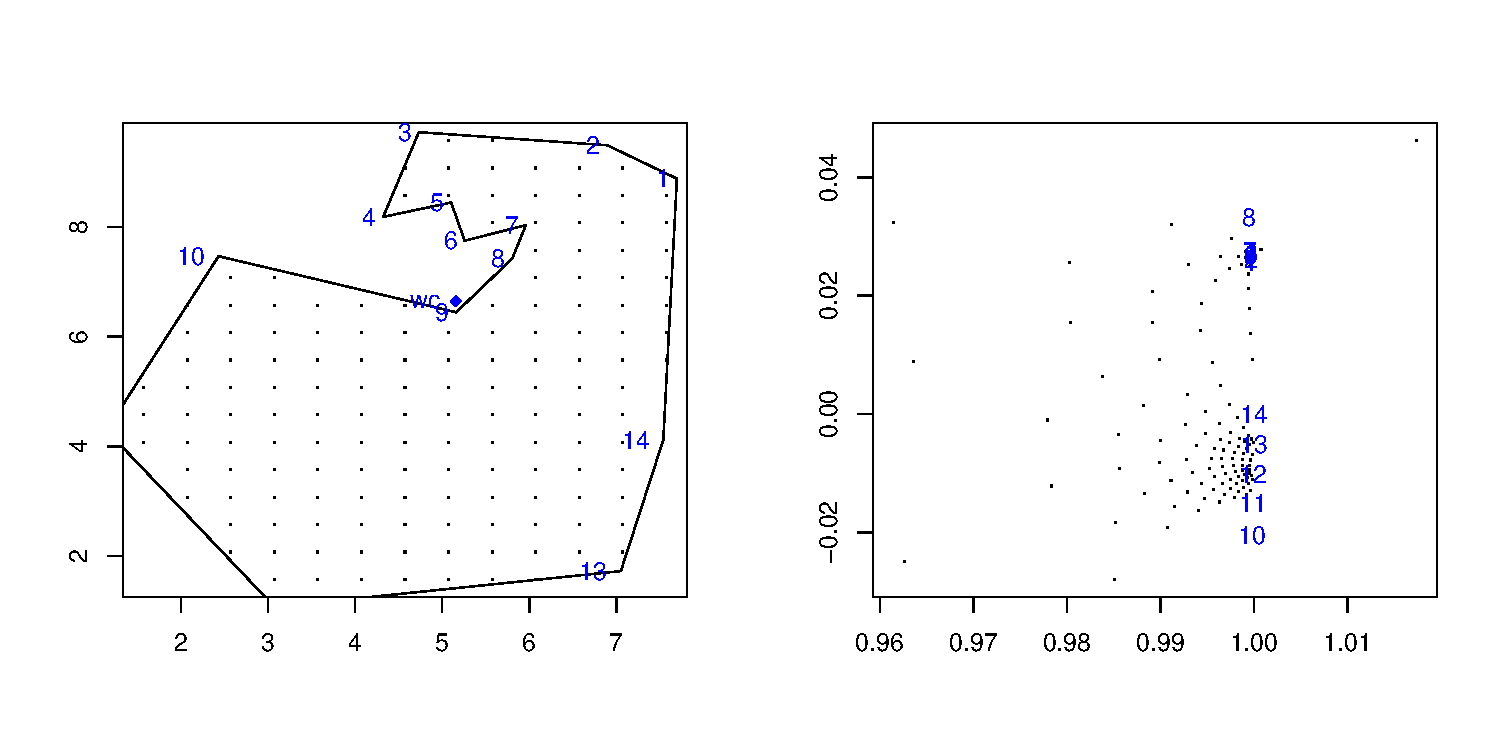
\includegraphics[scale=0.5]{figs/crowdeddisk.pdf}
\caption{An example of crowding. Notice how prevertices 1 through 8 are mapped to a single point in the right panel and their relative proximity in the left panel.}
\label{crowdeddisk}
\end{figure}

\subsection{Fixing crowding}

If the crowding is caused by $\Gamma$ being elongated then a  primitive fix is to map to an elongated domain such as the rectangle or plane. This approach is suggested in \cite{howell90} however, as they point out, this does not eliminate all crowding and problems can still occur when there are strongly acute peninsulae in the polygon. Mapping to an elongated domain also does not fix problems which occur when mapping from T- or H-shaped domains (so-called ``multiply elongated'' domains.)

In order to combat this problem more effectively, \cite{vavasis96} propose the CRDT (cross-ratios of the Delaunay triangulation) algorithm. Since each set of prevertices has $n-3$ degrees of freedom, there is a three parameter family of possible vertex arragements that all map to the same polygon, we would like to use the most stable of these \emph{embeddings}. The M\"{o}bius transformation relates the embeddings to one another.

We can extend this idea further by noting that the polygon is identical if additional vertices are added between the current ones, provided that the internal angle associated with the new vertex is $\pi$. These extra vertices also do not change the \sch formula since in \eqn{unitscmap} $\alpha_k=1$ for an angle of $\pi$. Adding these extra vertices allows us to control the aspect ratio of the map.

Finally, in the classical solution to the \sch parameter problem we enforce conditions on the side lengths and orientations of the polygon, instead we would now like to impose conditions about quadrilateral sections of the polygon and the diagonals of the polygon. We can do this by first triangulating the domain and then merging each pair of triangles into a quadrilateral. A measure is then defined (the \emph{cross-ratio}) which specifies a set of non-linear equations to be solved. These equations enforce the constraint that the cross-ratio in mapped polygon comes out correctly. 

Putting all of these ideas together gives the CRDT algorithm. We first add edges to the polygon with internal angle $\pi$ to remove enlongated parts of the domain and then triangulate the domain. Once the domain is triangulated we calculate the cross-ratio:

\begin{equation}
\rho(a,b,c,d) = \frac{(d-a)(b-c)}{(c-d)(a-b)},
\end{equation}

for each quadrilateral in the polygon. Then, analogously to \eqn{optimizeme} we set up a series of equations, specifying that the cross-ratios remain the same in the polygon and the transform of the rectangle back to the polygon. We then wish to solve for the values of $\rho$ for the original domain in the same manner as we solved for side lengths in the original problem. 

We can see in \fig{uncrowdeddisk} that when the CRDT method is used with a rectangular domain that the crowding has been alleviated. The point density, as well as vertex density seems to be more uniform than in \fig{crowdeddisk}.

% Uncrowded mapping diagram
\begin{figure} [tbp]
\centering
\includegraphics[scale=0.5]{figs/irregular-fixed-crdt.pdf}
\caption{The mapping of the irregular domain featured in \fig{crowdeddisk} using the CRDT method mapping to a rectangle. The crowding is now much less severe.}
\label{uncrowdeddisk}
\end{figure}

The downside of using CRDT is that it may add too many vertices to maintain the aspect ratio (\cite{driscoll05},) so the algorithm tends to take longer than the one specified in Section (\ref{algorithmsketch}) since it is $O(n^3)$. This is, of course, offset against the fact that the problem becomes tractable.

\bibliographystyle{plainnat}
\bibliography{sc-refs}

\end{document}
